%\documentclass[10pt,a4paper,final,oneside,openany,article]{memoir}
%\documentclass[letterpaper,a4paper,10pt]{article}
\documentclass[10pt,letterpaper,final]{article}
\usepackage[utf8]{inputenc}
\usepackage[british]{babel}
\usepackage{hyperref}
\setcounter{tocdepth}{3}
\usepackage[draft]{fixme}
\usepackage{abstract}
\usepackage{todonotes}
\usepackage{longtable}
\usepackage{amsmath}
\usepackage{pifont}

%% FONT
%\usepackage[T1]{fontenc}
%\usepackage{lmodern}
%\usepackage[urw-garamond]{mathdesign}
% Fonts configuration
%  - Palatino and Bitstream Vera Sans Mono for verbatim
\usepackage[T1]{fontenc}
\usepackage{palatino}
\usepackage[sc]{mathpazo} % Math font for Palatino
\usepackage{bera}
\linespread{1.05} % Palatino needs more leading (space between lines)
\usepackage{microtype}
\usepackage{graphicx} % ++
\usepackage{color}
\definecolor{kugrey}{rgb}{.4,.4,.4}
\usepackage{listings}
\usepackage{amssymb}
\lstset{ %
    language=Python,                % choose the language of the code
    frame=single,                   % adds a frame around the code
    keywordstyle = \footnotesize\ttfamily,
    commentstyle = \color{kugrey}\textit,
    stringstyle = \ttfamily,
    basicstyle   = \footnotesize\ttfamily,
    numberstyle=\tiny,
    sensitive = true,
}

%% odds and ends
%\chapterstyle{hangnum}
\setcounter{secnumdepth}{2}

%HEADINGS
\title{Constructing Models For Diagnosing Rare Diseases}

\author{Brian S. Mathiasen $-$ soborg@diku.dk \\
        Henrik G. Jensen $-$ henne@diku.dk\\
%        \\
%        Department of Computer Science\\
%        University of Copenhagen\\
%        Universitetsparken 1\\
%        DK-2100 Copenhagen, Denmark
}

\date{\today} %\today

%%
\begin{document}
\maketitle
\listoffixmes
%\tableofcontents


\begin{abstract}
In this paper we design and construct models for assisting physicians
with the task of diagnosing rare diseases. Using a prior knowledge of
rare diseases consisting of \textit{disease name, some symptoms} and
\textit{synonyms}, we utilize the \textit{Google Search Engine} to build
the model over several iterations. The models are constructed using
machine learning and natural language processing techniques by text
mining symptoms and features from abstracts and other relevant
paragraphs of text found in the search process.
\todo[inline]{Tests and results}

\end{abstract}
%%-----------------------------
%\newpage

\section{Preface}
The source code, this report and the previous project by
\cite{jensenandersen} is available at the repository:
\url{http://code.google.com/p/disease-crawler/}
%Installation and usage is exclusively the responsibility of the user.
The system is developed in Python version 2.6.6 on Ubuntu 10.10,
utilizing the following external modules:
\begin{itemize}
\item nltk \footnote{\url{http://nltk.org}}, Ubuntu repository module: \texttt{python-nltk}
\item numpy \footnote{\url{http://numpy.scipy.org}}, Ubuntu repository module: \texttt{python-numpy}
\item hcluster \footnote{\url{http://code.google.com/p/scipy-cluster/}}
\item lxml \footnote{\url{http://lxml.de}}, Ubuntu repository module: \texttt{python-lxml}
\item sqlite3, Ubuntu repository module: \texttt{python-sqlite}
\end{itemize}

\subsection{Expectations to the reader}
The reader is expected to have knowledge in Computer Science at a
Master's degree entry level.

It is expected that the reader has read the project
\cite{jensenandersen}.

We expect the reader to have knowledge of Natural Language Processing
techniques, in particular POS-tagging and phrase chunking. It is also
required to have knowledge of the foundations and overall philosophy of
Machine Learning.


\section{Introduction}
%\label{chap:introduction}
Physicians have expressed a need for aiding in the process of diagnosing
rare diseases \cite{googlingdiagnosis}, and point towards using the
Internet as a resource for information gathering, with particular focus
on utilizing Google or other popular search engines
\cite{googlechangemedicine} \cite{diagnosissearchengines}.

%The current process of automating this process relies heavily on static
%information, which is only expanded through manual interaction. \fxwarning{citation needed}
%\url{http://www.wrongdiagnosis.com/},
%\url{http://www.rarediseases.org/}, \url{http://www.orpha.net/}.

In this project, we investigate several methods for automating
information collection of specific features from rare diseases. The
project is mainly developing proof of concept models, on which a
practising physician can query a case report or a number of search terms
and get a list of disease predictions based on the knowledge of the
model.

The basic model is constructed given information of 3882 diseases, with
corresponding abstract or disease group information. This information,
together with the disease name and other relevant terms are used to
harvest the Internet for related information to expand the knowledge of
that particular disease.

A number of post-processing techniques are now applied to the basic
model to develop the final proof of concept models, based on different
characteristics and processing strategies.


% The models are sketched as
%follows:
%\begin{description}
%\item[Unigram] This model is similar to the model developed in the proje
%\item[Cleansed Model]
%\item[Unigram+NLP]
%\item[ICD10 model]
%\end{description}


%In order to increase the prediction precision, the model is expanded by
%harvesting information of some disease through a number of iterations on
%popular search engines. The harvested data is sanitised and irrelevant
%or low-information paragraphs are removed to reduce noise within the
%model. The prediction process is performed by, given a query, a number
%of diseases are returned that match the the query, in addition to
%ICD10\footnote{The International Statistical Classification of Diseases
%and Related Health Problems 10th iteration (ICD10) is a classification
%of diseases, signs and symptoms, classified by the World Health
%Organization (WHO).} code clusters and Natural Language Processing (NLP)
%based models. \todo[inline]{rewrite to make it crystal clear!}


%We use Natural Language Processing (NLP)
%provided through a Python library \cite{NLTK} to extract unique
%information from some description of the disease, and use Machine
%Learning to refine the search within the model.

%by assuming certain semantic and
%syntactic properties of symptoms and medically related phrases and
%terms.


\subsection{Limitations}
We have not developed a fully automatic system that with a simple
interface is able to take a query and return a prediction. The system
and models are developed as autonomous modules and have not yet been
fine-tuned or assembled as a complete program.


\subsection{Content outline of this document}
In section \ref{chap:previouswork} we will outline current and previous
work and briefly discuss the differences to this project.

In section \ref{chap:method} we will present an overview of the methods
used, and go into detail with the most important steps, by discussing
information harvesting, feature extraction, modelling and prediction.

% of each of
%the developed models.

In section \ref{chap:implementation} we will go into the implementation
details of the various models, highlighting the overall architecture and
pipeline of constructing the models, and discuss which methods are used
in each model.

% while
%explaining the more important parts of the architecture.

In section \ref{chap:test} we present the results from our tests, here
among blind tests, BMJ and Orphanet, further explained in section
\ref{chap:test}, comparing our results with previous similar projects.
We will discuss the results with a strong focus on statistical analysis.

Finally, in chapter \ref{chap:conclusion} we will conclude the project,
and discuss major implications and advantages of the system, methods and
tests. We will finally propose a number of topics for future work.


%In the following we will present and highlight current and previous work
%within this domain. In chapter 3, we will discuss our method
%methodically, with particular focus on construction of model and feature
%extraction and post processing of harvested information.
%Then we will explain how we tested the system and argue statistical
%significances by comparing to previous work, as well as assessing the
%viability of our system as it is.
%Finally we will conclude our paper and discuss implications and other
%thoughts relevant to our method, while also proposing a number of topics
%for future work.

\section{Previous Work}
\label{chap:previouswork}
The article \cite{googlingdiagnosis} proves the viability of using
Google as a diagnosis aid, despite the tests being done manually with
little consideration with regard to automation or test reliability and
validity.

\cite{jensenandersen} proposed a system for diagnosing rare diseases
using vector space models and text mining. They showed a potential in
automating such a process, but their results were not statistically
significant. Their system did not rely on prior knowledge of particular
diseases, but still showed that around 60\% of the tests were
satisfactory (correct disease located within the top 20 predictions).

Our colleagues Radu Dragusin and Paula Petku from the department of
Computer Science at Copenhagen University investigate a related way of
automating information gathering to what we are presenting. However, as
this is a work in progress we do not have access to further information
at this point in time \cite{radupaula}.



%Our system will move on to the next step and introduce intelligent
%automation through a number of predefined criteria and utilizing several
%machine learning and natural language processing techniques.


%The editorials \cite{googlechangemedicine} and
%\cite{diagnosissearchengines} suggest Google and search engines in
%general as being a very strong player in the task To perform the initial
%testing we mimicked the previous project where a TF-IDF\footnote{Term Frequence - Inverse Document Frequence.} matrix was build
%using information (abstracts,titles, keywords) gathered form Pubmed. The
%knowledge of search engines being a valuable source of information is
%apparent, but the shear amount of misinformation and noise from regular
%searches make such a method in it’s current incarnation unreliable and
%error prone.\fxwarning{citation needed} \todo[inline]{Omformuler,
%præciser!}


%(Our goal is to refine and provide means for filtering out this noise
%and focus on harvesting information from related material with reference
%to the original search terms as well as specific criteria for the text
%mining process.)


%Inspiration for a system: Online Search Engine specialised for
%diagnosing stuff etc.
%http://www.healthline.com/symptomsearch

%This system is based on simple searches that relies on an already
%established database of diseases with appropriate meta-information. The
%user is able to search for symptoms and can narrow down the search by
%adding several symptoms. The system will then present a list of possible
%diseases according to some relevance criterion.

%(It is an end-user focused system, while our system will be a back-bone
%focused system, attempting to establish a model on which queries may be
%imposed. It will as such automate the information collection based on
%several machine learning and natural language processing techniques
%appropriate for the needs.)


%Google Health: http://www.google.com/intl/en-US/health/about/index.html


%Article by practising doctor on “do’s and don’t’s when using Google as
%diagnosis aid”:
%http://vitualis.wordpress.com/2007/02/26/google-based-medicine/


\section{Method}
\label{chap:method}
Data received from Orphanet, an online database of information
specialised on rare diseases, is initially used as prior knowledge to
harvest additional information from the Internet.


%As one of the premises of the project was to introduce prior knowledge
%of the disease model, we needed to process our available data. We were
%given a large corpus of data from Orphanet \ref{app:orphanet},
%consisting of \texttt{\{orphanum, disease name, disease
%description/abstract, maybe author and date\}} for each disease in the
%data set.\todo[inline]{Rewrite this nonsense.}


The data is processes similar to what is described in
\cite{jensenandersen}, and will thus be used to bootstrap the knowledge
of each disease, allowing us to iterate and harvest additional
information using various harvesting techniques roughly covering the use
of the \textit{Google} search engine to collect an array of websites
given a query relevant to the disease (disease name and a possibly a
number of keywords). For each website, we will collect paragraphs and
save it for further processing given an acceptance threshold.

%For each
%accepted paragraph we use NLP to identify candidates for relevant terms
%and phrases that will then be used to expand the model. 

The abstract flow model is shown in figure \ref{fig:flow}.

\begin{figure}[htp!]
\begin{center}
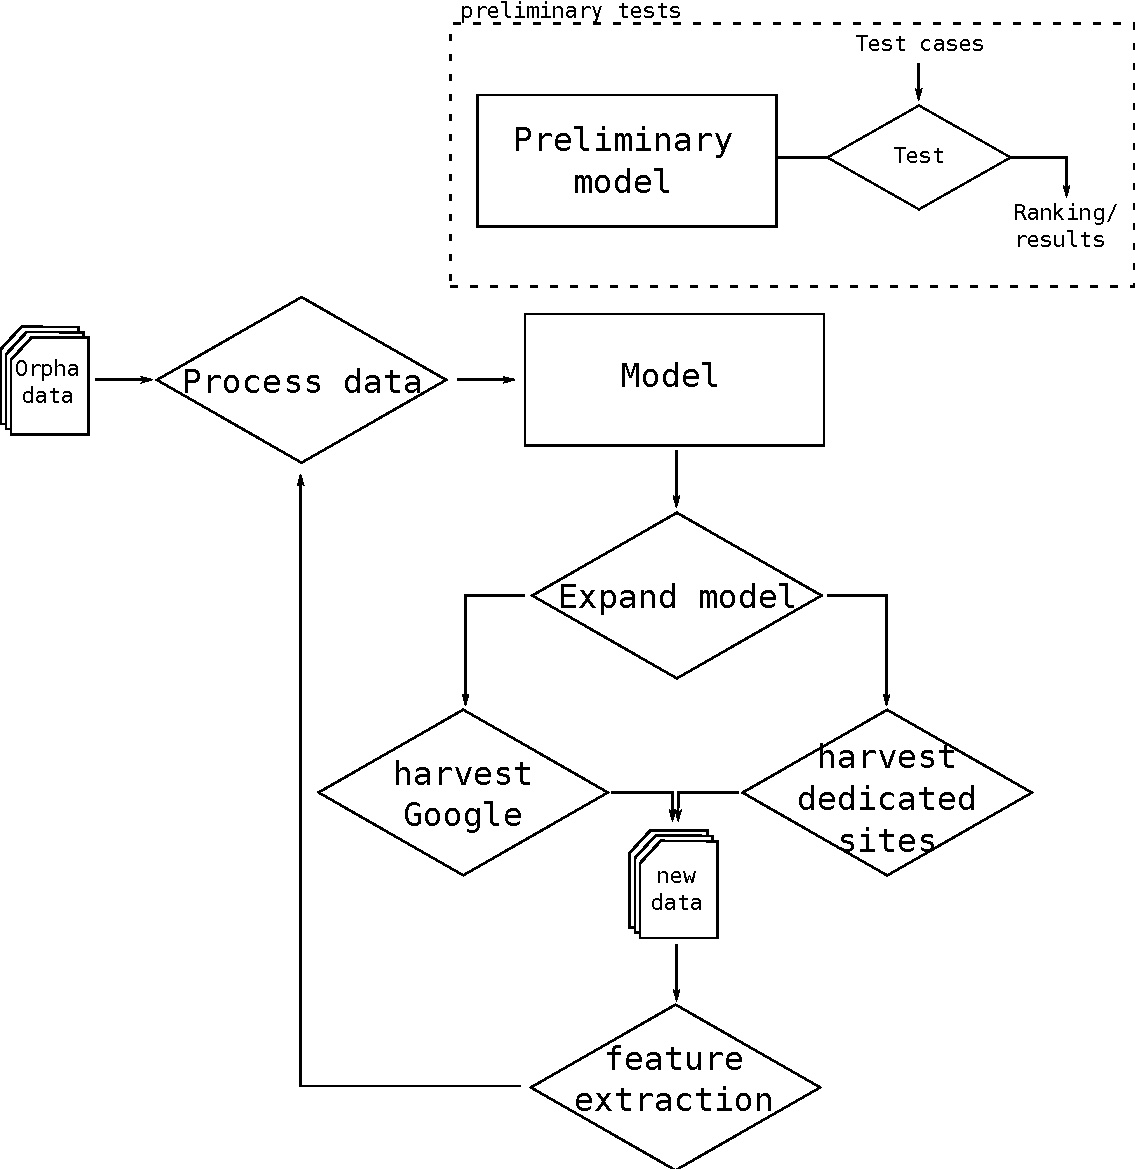
\includegraphics[scale=0.4]{images/pipeline}
\caption{Systems diagram}
\label{fig:flow}
\end{center}
\end{figure}

As several individual models are being constructed, we will highlight
the most important cornerstones of all the methods used independently
across all the models.
We initialise by explaining how the basic model is constructed and how
we have refined it into a number of proof of concept models.

%\todo[inline]{Something N-gram machine learning here.}

\subsection{Building the basic model}
The basic model is built using the prior information available
from Orphanet. The TF-IDF model is essentially identical to the model
constructed in \cite{jensenandersen}, except our prior information is
not harvested and thus prone to be noisy, but consists of validated
abstracts and titles for each disease.

%To perform the initial testing we mimicked the setup of
%\cite{jensenandersen} where a TF-IDF matrix was build using information
%(abstracts,titles, keywords) gathered form Pubmed.

%A sparse term-disease matrix (similar to the well-known term-document
%model) is built over the abstracts received from Orphanet. 
Each row in the matrix thus represents a feature vector of a disease
with the features being a list of term frequencies. Prior to the
creation of the matrix, the terms were stemmed (using the Porter
stemming algorithm \cite{porterstemming}) and stopwords \footnote{The stopwords are defined by a
list of 127 English words provided by the Python NLTK library
(\texttt{nltk.corpus.stopwords.words("english")}} are removed along
with non-alphanumerical \footnote{Symbols not represented in the Danish
Alphabet} symbols.

Stemming a word involves reducing it to it's most basic form or root,
removing morphological and inflectional endings from the words. E.g.
walking, walker, walks have the affixes \textit{-ing}, \textit{-er} and
\textit{-s}, with the common root \textit{walk}.


The term-disease matrix is then processed using the
TF-IDF model (as originally proposed by \cite{tfidf}) along with
additional logarithmic smoothing of the $tf_{t,d}$-parameter to flatten
term-burstiness (\cite{burstiness}) \todo[inline]{Why is this smoothing good?}.

The TF-IDF model is thus constructed as such:
\[
w_{t,d} = log(tf_{t,d}+1)\cdot log\frac{|D|}{|\{d'\in D|t\in d'\}|}
\]
where $tf_{t,d}$ is term frequency of term $t$ in disease $d$, $|D|$ 
the total number of diseases in the disease set, and $|\{d'\in D|t\in
d'\}|$ the number of diseases containing the term $t$.

To compare the precision of the new model to the previous, we made the
same queries to the model using the same scoring-scheme to obtain a rank
for each disease. The rank of each disease represents the precision of
the model.

A query is given, stemmed and stopwords are removed. Each
disease-vector that contain one or more of the queried terms is given a
score which is based on a summation of each of the weights of the
queried terms relevant to the disease.
\[
s_{d} = \displaystyle\sum\limits_{t_1}^{t_n} w_{t,d}\quad t \in Q
\]

\paragraph{Example}
Consider four diseases, each consisting of up to three terms:
\[
d_{0} = \{t_{2}\}, d_{1} = \{t_{0}, t_{2} \}, d_{2} = \{t_{2} \}, d_{3} = \{t_{0}, t_{1}, t_{2} \}
\]

Then the TF-IDF matrix is constructed, at this point ignoring the
logarithmic smoothing:

\[ \mathbb{M} = \left| \begin{array}{ccc}
0 & 0 & 0.25 \\
0.5 & 0 & 0.25 \\
0 & 0 & 0.25 \\
0.5 & 1 & 0.25  \end{array} \right|.
\]

In this case the queries terms correspond with all represented terms of
$\mathbb{M}$, then the summation of the weights of the queries terms are
given as

\[ \mathbb{S} = \left| \begin{array}{c}
0.25 \\
0.75 \\
0.25 \\
1.75 \end{array} \right|.
\]
Thus the bottom entry with a score of $1.75$ is the model's prediction
of the correct disease/diagnosis. \ding{111}\newline


Though the model used in \cite{jensenandersen} was based on large
amounts of information gathered from PubMed, our tests showed that we
could obtain close to the same precision solely based on the abstracts
from Orphanet.

(This may indicate a large amount of noise being present
in the data set used in the previous project where the information (or
model) of each disease was based on non-validated abstracts from PubMed
using customised queries.)\fxwarning{rewrite}

The results can be seen in appendix
\ref{app:preliminary_results}.


\subsection{Harvesting data}
Harvesting additional data to expand the basic model is done using the
Google search engine. For each site returned from the query, i.e.
disease name and a number of keywords from disease abstract, paragraphs
are extracted to measure the relevance of that paragraph compared to the
corresponding abstract from Orphanet. The comparison is measured using a
cosine distance measure of two term vectors representing known
information, $\textbf{s}$ and a harvested paragraph of information
$\textbf{p}$ which is defined as
%\footnote{Definition extracted from the
%HCluster cosine source code definition.}:
\[
similarity(\textbf{s}, \textbf{p}) = \frac{1 - sp^T}{||s||_2 ||p||_2}
\]
Which, using algorithms provided by the HCluster
\footnote{\url{http://code.google.com/p/scipy-cluster/}} library returns
a score between $0$ and $1$, where 0 is complete correlation and 1 is
no correlation. The acceptance threshold for paragraphs collected for
further processing is set to $0.8$. This number is used based on a
number of anecdotal tests showing a reasonable amount of relevant
information, where $0.9$ would introduce too much noise, and $0.7$ being
too strict.

It is observed that many of the harvested paragraphs are literature
references and should be considered noise, due to it's low information
value.
These paragraphs are structured by a listing of names followed by a
title and other meta information and the filtering process is done by
utilizing the named entity chunker provided by the NLTK library, e.g.
\textit{``Post MC, Letteboer TGW, Johannes JM, et al. A pulmonary
right-to-left shunt in patients with hereditary hemorrhagic
telangiectasia is associated with an increased prevalence of migraine.
2005;128(4):2485-9. Chest [Medline]''}. It is apparent that this paragraph
is a literature reference, and while the title itself contains terms
that could be relevant for later symptom extraction, it has been decided
that this entire paragraph is considered noise, and will thus be
filtered.

%\todo[inline]{Write pseudocode for this harvesting and paragraph
%selection procedure}


%The comparison consists of constructing a $2 x n$ matrix, for $n$ being
%the number of unique terms in both texts, after which the cosine
%similarity measure is calculated and accepted paragraphs pushed onto
%further processing.

\subsection{Feature Extraction}
Feature extraction is used as a means to extract unique or otherwise
relevant information from a document regarding a specific disease. The
purpose is to built a phrase document matrix similar to the above
mentioned TF-IDF matrix, i.e. a \textit{Phrase Frequency - Inverse
Document Frequency} matrix (PF-IDF). We hypothesise that extracting
terms and phrases directly relevant to the essence of a particular
disease may reduce noise of irrelevant but infrequent words, that would
otherwise have a high score, compared to the old TF-IDF model. The
challenge lies in the strictness of the grammar that produces symptom
candidates.

The process of extracting features consists mainly of POS-tagging and
subsequent chunking into phrases, involving a nested iteration through
an array of POS-taggers and subsequent chunking by exploiting certain
syntactic and semantic properties of sentences.

\subsubsection{POS-tagging}
The POS-tagging procedure, which is a variant of a braubt
\footnote{Brill, Regexp, Affix, Unigram, Bigram, Trigram} tagger built
using the following strategies, is listed here in decreasing order of
complexity and context exploitation:
\begin{description}
\item[Brill tagging] The Brill \cite{Brill:1992:SRP:974499.974526}
tagger starts by running an initial tagger, and then improves the result
by applying a list of transformation rules. These rules are
automatically learned from the training corpus.
\item[Affix tagging] The affix tagger is similar to the unigram tagger.
It takes some fixed-size substring of a word and finds the most likely
tag for that substring.
\item[Trigram tagger] This tagger works like the bigram tagger, except it
uses two pieces of information. N-gram taggers assigned tags to tokens
depending on the $N - 1$ preceding tags.
\item[Bigram tagging] A bigram tagger work similarly to the unigram
tagger, except it finds the most likely tag for each word given the
preceding tag.
\item[Unigram tagging] A unigram tagger finds the most likely tag for each word
in the training corpus and uses that information to assign tags to new
tokens.
\item[Maxent treebank pos tagger] A classifier based pos tagger, trained
on the maxent treebank training set \footnote{Available through the NLTK
data collection.}.
%\item[Regexp tagging] This tagger assigns tags to tokens based on regular
%expessions.
\end{description}
%Which we will refer to as a batbum tagger. 
Notice, that opposed to the
braubt tagger we do not use a regular expression tagger but utilize a
classifier based maxent treebank pos tagger. The goal of using this many
taggers is to encode as much information about a sequence of words to
get proper tagging based on the context. When a tagger fails to identify
a context for a given sequence, a less complex tagger takes over and
attempts to tag, and thereby runs through the list of taggers and
finally ending with the maxent treebank pos tagger.

The taggers are trained on the Brown corpus \footnote{Available through
the NLTK corpus collection.}. While the corpus is not directly
applicable in a medical domain, and realising the importance of training
on representative data, we have observed anecdotal increase in precision
using the above taggers in sequence, as opposed to using much simpler
strategies, such as regular expression or dictionary based taggers.

\subsubsection{Chunking}
In order to iterate and collect information to expand the modelling of
relevant terms and phrases we use NLP to identify symptoms and medical
terms (here-on referred to as just symptom) from abstracts and
paragraphs harvested. 

%Identifying unique symptoms to use in parallel
%with the basic model will 

%and correlate with
%other documents describing the same disease will increase the knowledge,
%or further substantiate pre-existing knowledge of that disease. The
%ultimate goal of this strategy is to expand the basic model as a means
%to focus on medically relevant information.

Through a number of anecdotal observations it is experienced that
symptoms are usually described as zero or more adjectives or verbs
followed by one or more nouns. These phrases can be caught using a
regular grammar defined through the Python NLTK library
\footnote{\url{http://nltk.org/}} as such:
\begin{lstlisting}
grammar = """SYMPTOM: {(<JJ|VB(N|G|D)>*<N(P|N)>+)}"""
\end{lstlisting}
This will catch candidates such as \texttt{bleeding diathesis}, but will
also match non relevant terms such as \texttt{addition}.
 based
%The premise for the construction of this grammar is substantiated
%through anecdotal manual observations of a handful of abstracts from the
%orphanet data set, and utilized under the assumption that it will
%increase the amount of medically relevant terms as opposed to simply
%catching all combinations matching the \texttt{SYMPTOM} grammar above.

As an example, the grammar applied to the sentence
\textit{``Hermansky-Pudlak syndrome type 2 is a type of Hermansky-Pudlak
syndrome, a multi-system disorder characterized by oculocutaneous
albinism, bleeding diathesis and neutropenia.''} \footnote{Excerpt from
the Hermansky-Pudlak syndrome abstract from the Orphanet data set.}
yields the following POS-tagged syntax tree:
\begin{lstlisting}
(S
  (SYMPTOM Hermansky-Pudlak/JJ syndrome/NN type/NN)
  2/CDmatrix
  is/BEZ
  a/AT
  (SYMPTOM type/NN)
  of/IN
  (SYMPTOM Hermansky-Pudlak/JJ syndrome/NN)
  ,/,
  a/AT
  (SYMPTOM multi-system/NN)
  disorder/IN
  characterized/VBN
  by/IN
  (SYMPTOM oculocutaneous/JJ albinism/NN)
  ,/,
  (SYMPTOM bleeding/VBG diathesis/NN)
  and/CC
  (SYMPTOM neutropenia/NP)
  ./.)
\end{lstlisting}
of which we are particularly interested in the \texttt{SYMPTOM}
subtrees. For each existing paragraph or abstract for a given disease, a
list of phrases and terms are returned for further processing.

While the grammar does not explicitly collect symptoms or medical terms,
we attempt to filter out noise by ruling out candidates that are not
represented in the above mentioned harvested symptom database of which
a PF-IDF matrix can be built and used together with the basic model.
Chapter \ref{chap:implementation} explains how these models are
implemented and utilized.

%Additionally, while having collected a number of symptom candidates
%$\mathbb{S}$ from some document or paragraph, we calculate the number of
%unique terms and return the candidates $\mathbb{S'}$, that appear more
%than once or is a substring of other candidates. Consider the set of
%candidates already filtered against the before mentioned database,
%$\mathbb{S} = $ \texttt{\{bleeding diathesis, bleeding tendency,
%bleeding, sleep apnae\}}. The system will then count \texttt{bleeding}
%as well as \texttt{bleeding diathesis} and \texttt{bleeding tendency} as
%that is a substring of the other two. We will thus accept the symptoms
%$\mathbb{S'} = $ \texttt{\{bleeding diathesis, bleeding tendency,
%bleeding\}}.


%% \todo[inline]{rewrite}
%%Using the rule:
%%\begin{equation}
%% s_{j}, s_{i} \in \mathbb{S'} ||s_{j}|| > 1 \wedge||s_{i}|| \wedge s_{j} \subset s_{i}, \texttt{for } s_{i}, s_{j} \in \mathbb{S}
%%\end{equation}
%%\todo[inline]{valider formel}
%Anecdotal observations during the development phase of this module
%showed that returning terms and substrings of terms using this strategy
%increased the amount of relevant symptoms, and seemed to decrease the
%amount of noise generated in the symptom harvesting process.

\subsection{Utilizing ICD10 Codes}
For approximately 50\% of the diseases in our existing models, an ICD10
label is attached. This label is a categorization




\section{Implementation}
\label{chap:implementation}
As mentioned previously, a number of different models are constructed to
give a better foundation for comparison between the models. In
particular, a \textit{basic} model - cleansed from some noise, an
\textit{NLP+basic} model and finally an \textit{ICD10 code} based model
is constructed and ultimately used for testing and comparison.

\subsection{Basic}


\subsection{NLP+Basic}


\subsection{ICD10 code}


\section{Tests}
\label{chap:test}
In the following, we will distinguish the different methods and models
as such:
\begin{description}
\item[Old model] Refers to the model constructed in
\cite{jensenandersen}
\item[New model] Refers to the model constructed using the Orphanet data
set.
\item[New model(cleansed)] Refers to the model constructed using the
Orphanet and harvested data set, cleansed for low information
paragraphs.
\item[New model(NLP)] Refers to the model constructed by extracting
phrases using NLP methods.
\end{description}

The test sets are described as such:
\begin{description}
\item[Blind tests] These tests are originally blind tests from
\cite{jensenandersen} provided by a practising physician only as a list
of terms, and was later correlated with the proper diagnosis after the
model returned a prediction.
\item[Orpha tests] Tests provided by \todo[inline]{how did we get these tests?}
\item[BMJ tests] Selected tests from \cite{googlingdiagnosis}, yielding
only tests that are labelled as 'rare diseases' \footnote{A disease is
considered a rare disease if it is listed in
\url{http://rarediseases.org}.}.
\end{description}


%We have chosen to base our tests on known test cases, from in particular
%those mentioned in \cite{jensenandersen}, \cite{googlingdiagnosis} and
%tests listed in appendix \ref{app:tests}. We will then consider the
%significance across the results and introduce the independent variable
%\texttt{method} with the values \texttt{\{manual, semiautomatic,
%automatic\}}, where \texttt{manual} is the method used in
%\cite{googlingdiagnosis}, \texttt{semiautomatic} is the method used in
%\cite{jensenandersen} and finally \texttt{automatic} is the method
%described in this paper.

\subsection{Kruskal Wallis Test Statistics}
The tests are compared using the prediction ranking of the correct
diseases in the various models. There is no evidence that the data
samples are normally distributed, which is a prerequisite in the
commonly used Student's T test, we will use the one-way Kruskal-Wallis
\cite{kruskalwallis} test for multiple groups (models) to determine the
statistical significance as this does not rely on that assumption. It
does, however, assume the observations come from distributions of the
same shape, e.g. if one distribution is skewed left($<0$) and the other
is skewed right ($>0$), the test will be likely to yield inaccurate
results.

We will calculate the Kruskal-Wallis test statistic
\[
H_{stat} = \frac{12}{n(n+1)}\sum\limits_{i = 1}^{k} \frac{R^{2}_{i}}{n_{i}} - 3(n+1)
\]
where $n_{i} (i = 1, 2, ..., k)$ represent the samples for each of
the k groups. $R_{i}$ is the sum of ranks for group $i$. The ranks are
acquired by sorting the sample values in ascending order and ranking
from $1$ to $\sum n_{i}$, giving identical sample values the mean of the
ranks tied for.

$H_{stat}$ approximates a chi-square ($\chi^2$) distribution with k-1
degrees of freedom if the null hypothesis of equal populations is true,
when the number of samples is at least 5.

To assess whether the null hypothesis can be rejected, we use table
values of chi-square
\footnote{\url{http://www.ma.utexas.edu/users/davis/375/popecol/tables/chisq.html}}
with 1 degree of freedom ($k-1$) with an acceptance threshold of $\alpha
= 0.05$:
\[
\chi^2_{0.05}(df=1) = 3.84
\]

%The critical value $H_{crit}$ can now be calculated as the chi-square
%percent point function (CHIPPF).

% or CHIINV as provided by \textit{Open
%Office 3.2} for $\alpha = 0.05$. \todo[inline]{find a proper formula for
%CHIINV: \url{http://en.wikipedia.org/wiki/Inverse-chi-square_distribution}}

For our purpose, we will be looking at a right-tail test, yielding the
hypotheses:
\begin{itemize}
\item $H_{0}$ the samples come from the same distribution, i.e. the models yield identical results ($u = a$)
\item $H_{1}$ the new model yield significantly better results than the old ($u > a$)
\end{itemize}
\todo[inline]{reconsider using this hypothesis explanation gibberish}

Therefore, we can reject the null hypothesis, if $H_{stat} > \chi^2$,
and accept that there is a difference between the groups.

The results of the significance tests are presented in the following.

% We will measure statistical significance
%across the models using the Mann-Whitney U test. Alternatively, we will
%identify if the data samples are normally distributed using the Skew and
%Kurtosis test, and accordingly use the Student's T test where
%appropriate, as this test assumes normally distributed samples.

\subsection{Significance testing results}
In this section, we will highlight our most important results from the
previously described models and test scenarios.

\begin{table}[here]
\begin{center}
\begin{tabular}{lll}
    \textbf{Data set} & & \textbf{Orphanet} \\ \hline\hline
    \textbf{Parameter} & \textbf{Old model} & \textbf{New model} \\ \hline
    Skew & 3.34 & 5.26 \\
    $R_{i}$ & 1161 & 435 \\
    $n_{i}$ & 28 & 28 \\ \hline\hline
    \textbf{Test Parameter} & & \textbf{Value} \\ \hline
    $n$ && 56  \\
    k && 2  \\
    df && 1  \\ \hline \hline
    \textbf{Result} & & \\\hline
    $H_{stat}$ & & 35.38 \\
    $H_{crit}$ & & 3.84 \\
    \label{tab:orpha_old_new}
\end{tabular}
    \caption{Results from the Kruskal Wallis significance test of the
    Orphanet tests on the old and new model.}
\end{center}
\end{table}

%using the dependent variable \texttt{prediction},
%that describes the position of the correct disease. I.e. 
%the best result is 1 and worst result is $n$ where $n$ is the number of
%known diseases in the models.

%The results are described in table \ref{tab:results1} below.
%\begin{center}
%	\begin{tabular}{llll}
%		Case number & Old model & New model(cleansed) & New model(NLP) \\ \hline
%		1 &  &  &  \\
%		2 &  &  &  \\
%		3 &  &  &  \\
%		4 &  &  &  \\
%		5 &  &  &  \\
%	\end{tabular}
%	\label{tab:results1}
%\end{center}

Note that, for the manual googling method, the results presented in
\cite{googlingdiagnosis} only considered binary results depicted as
'Yes' if they predicted the diseases and 'No' otherwise. There is no
ranking of where the correct was found from a number of possibilities,
in contrary to \cite{jensenandersen} and this project.




\section{Conclusion}
\label{chap:conclusion}
We have investigated the possibility of using the Google search engine,
as a means to gather additional information in order to expand knowledge
of a range of diseases. We have shown that the information gathered
along with prior information supplied through Orphanet abstracts yields
significantly better results compared to previous work \ref{tablet1}
\ref{tablet2} \ref{tablet3}.

By using NLP techniques we have refined the data harvested using the
Google search engine and shown significant improvements over using the
non-refined data \ref{tablesomething}. We have also constructed models
by using NLP feature extraction, but these have shown to yield worse
results, even in combination with the cleansed unigram model. The major
problem with the NLP model was the fact that the symptom extraction
failed to extract representative phrases and terms from documents and
abstracts and suggests a poor choice of or too strict chunking
procedure.

\todo[inline]{further discussion}




\subsection{Future Work}
Symptom extraction is a complex problem that requires the system to have
a substantial knowledge of not only symptoms, but also what is not
considered medically relevant. It requires an intelligent model to
determine whether a phrase is a symptom, medical term or not. Look into
ways of constructing a model that is able to predict whether a phrase
is medically relevant to use in the model or not.

A method that may improve symptom extraction is to utilize clustering
algorithms, but will, in turn of allowing us to directly measure the
performance of the system (training and testing), require a substantial
amount of preparation by annotating a large corpus of documents for
constructing a reasonable amount of data. In this project we have only
succeeded in harvesting phrases that \textit{are} medical terms and
symptoms, but have failed to harvest or construct an equally sized data
set consisting of terms that are \textit{not} related to medicine.

Querying for a disease given a set of keywords can be erroneous if the
terms are misspelled. Consider expanding the system to use use fuzzy
searches to correct for misspelling variations on keywords.

The model construction is rigid and undynamic once the initial model
construction is completed. That is, once a satisfactory amount of data
has been collected, the model is built and may only be expanded through
a complete reconstruction of the model. Consider ways to dynamically
expand the model, to support adding new information to any existing
disease, but also allow for expanding the model with new diseases.

Look into options of allowing the model to automatically identify new
diseases and automatically determining when information is found can
increase the knowledge of some disease, and add this information to the
model accordingly.


\renewcommand\bibname{References}
\bibliography{bib}
\bibliographystyle{apalike}

\newpage
\appendix
\section{Preliminary Tests}
\label{app:preliminary_results}

The results of the tests of the old mode, as explained in
\cite{jensenandersen}, and the model based on abstracts from Orphanet,
with no further processing.

%Despite the larger amount of information gathered in the old model,
%there is little difference in the results (Note that the Orphanet tests
%are fit to the new model which were build upon the same abstracts
%as the test queries in \ref{tab:results_orphanet}!). This indicates a
%large amount of noise in the data gathered in the old model.

%\vspace*{-3cm}
\subsection{Orphanet tests}
%\vspace*{-6cm}
\begin{center}
\begin{small}
	\begin{longtable}{|p{3.5cm}|p{4.5cm}|p{1.8cm}|p{1.8cm}|}	\hline
	\textbf{Disease}  & \textbf{query} & \textbf{Rank (new model)} & \textbf{Rank (old model)} \\
    \hline\hline
    Apparent mineralocorticoid excess & early-onset, severe hypertension, associated, low renin levels, hypoaldosteronism & 1 & 10\\    \hline
    Rubinstein-Taybi syndrome  & congenital anomalies, intellectual deficit, behavioural characteristics & 1 & 91\\    \hline
    Cholestasis - lymphedema  (Aagenaes syndrome) & chronic severe lymphoedema, severe neonatal cholestasis, lessens during early childhood and becomes episodic & 1 & 18\\    \hline
    Aase-Smith syndrome  & congenital malformations: hydrocephalus, cleft palate, severe joint contractures & 2 & 10\\    \hline
    Achondroplasia  & short limbs, hyperlordosis, short hands, macrocephaly, high forehead and saddle nose  & 1 & 5\\    \hline
    Acalvaria  & missing scalp and flat bones over an area of the cranial vault  & 1 & 87\\    \hline
    Acrodysostosis & abnormally short and malformed bones of the hands and feet (peripheral dysostosis), nasal hypoplasia and mental retardation & 1 & 80\\    \hline
    Acromegaly & progressive somatic disfigurement (face and extremities) and systemic manifestations & 1 & 106\\    \hline
    Biliary atresia & biliary obstruction of unknown origin, neonatal period & 1 & 3\\    \hline
    Bronchiolitis obliterans with obstructive pulmonary disease & inflammatory and fibrosing thickening of bronchiolar walls, airflow obstruction & 1 & 8\\    \hline
    Cholera & severe diarrhea and vomiting & 1 & 65\\    \hline
    Choroideremia & progressive degeneration of the choroid, retinal pigment epithelium (RPE), and neural retina & 1 & 17\\    \hline
    Coats disease & abnormal development of retinal vessels (telangiectasia) with a progressive deposition of intraretinal or subretinal exudates & 1 & 1\\    \hline
    Omphalocele-cleft palate syndrome, lethal & omphalocele and cleft palate & 2 & 3\\    \hline
    Darier disease & keratotic papules in seborrheic areas and specific nail anomalies & 1 & 2\\    \hline
    Ichthyosis - hepatosplenomegaly - cerebellar degeneration & ichthyosis, hepatosplenomegaly and late-onset cerebellar ataxia & 5 & 7\\    \hline
    Emery-Dreifuss muscular dystrophy & muscular weakness and atrophy, with early contractures of the tendons and cardiomyopathy & 1 & 1\\    \hline
    Costello syndrome & postnatal growth retardation, coarse facies, intellectual deficit, skin anomalies and cardiac abnormalities & 1 & 2\\    \hline
    Fibrodysplasia ossificans progressiva & congenital malformation of great toes, progressive, disabling heterotopic osteogenesis in predictable anatomical patterns & 1 & 1\\    \hline
    Acropectorovertebral dysplasia & fusion of the carpal and tarsal bones, with complex anomalies of the fingers and toes & 1 & 3001\\    \hline
    Osteogenesis imperfecta & increased bone fragility and low bone mass & 1 & 2\\    \hline
    Primary biliary cirrhosis & injury of the intrahepatic bile ducts & 6 & 10\\    \hline
    Hennekam syndrome & lymphoedema, intestinal lymphangiectasia, intellectual deficit and facial dysmorphism & 1 & 4\\    \hline
    Hyperlysinemia & elevated levels of lysine in the cerebrospinal fluid and blood & 1 & 85\\    \hline
    Jackson-Weiss syndrome & tarsal and/or metatarsal coalitions and variable craniosynostosis, accompanied by facial anomalies, broad halluces and normal hands & 1 & 40\\    \hline
    Jalili syndrome & amelogenesis imperfecta and cone-rod retinal dystrophy & 5 & 39 \\    \hline
    Jeune syndrome & narrow thorax and short limbs & 1 & 2\\    \hline
    Myeloma, multiple & overproduction of abnormal plasma cells in the bone marrow and manifested by skeletal destruction, bone pain, and presence of abnormous immunoglobulins & 1 & 3\\    \hline
    Trichodental syndrome & fine, dry and short hair with dental anomalies & 1 & 60\\    \hline
    \end{longtable}
    %\label{tab:results_orphanet_pre}
\end{small}
\end{center}

\subsection{BMJ ('Googling for a Diagnosis') tests }

\begin{center}
\begin{small}
	\begin{tabular}{|p{3.5cm}|p{4.5cm}|p{1.8cm}|p{1.8cm}|}
	\hline
	\textbf{Disease}  & \textbf{query} & \textbf{Rank (new model)} & \textbf{Rank (old model)} \\
    \hline\hline
    Cushing syndrome & hypertension, adrenal, mass & 3 & 2 \\    \hline
    Eosinophilic granuloma & Hip, lesion, older, child & \textit{Not in the model} & 598 \\    \hline
    Ehrlichiosis & fever, bilateral, thigh, pain, weakness & \textit{Not in the model} & 512 \\    \hline
    Neurofibromatosis type 1 & multiple, spinal, tumours, skin, tumours & \textit{Not in the model} & 30 \\    \hline
    Hereditary pheochromocytoma-paraganglioma syndrome & hypertension, papilledema, headache, renal, mass, cafe, au, lait & 10 & 414\\    \hline
    Creutzfeldt-Jakob disease & ataxia, confusion, insomnia, death & 196 & 7\\    \hline
    Churg-Strauss syndrome & Wheeze, weight, loss, ANCA, haemoptysis, haematuria & 3 & 2\\    \hline
    Dermatomyositis & myopathy, neoplasia, dysphagia, rash, periorbital, swelling & 63 & 4\\    \hline
    Cat-scratch disease & renal, transplant, fever, cat, lymphadenopathy & 1 & 1\\    \hline
    Toxic epidermal necrolysis (TEN) & bullous, skin, conditions, respiratory, failure, carbamazepine & 1 & 4\\    \hline
    MELAS syndrome & seizure, confusion, dysphasia, T2, lesions & 2 & 27\\    \hline
    Brugada syndrome & cardiac arrest sleep & 3 & 7\\    \hline
	\end{tabular}
\label{tab:results_bmj_pre}
\end{small}
\end{center}

\subsection{Blind tests}

\begin{center}
\begin{small}
	\begin{tabular}{|p{3.5cm}|p{4.5cm}|p{1.8cm}|p{1.8cm}|}
	\hline
	\textbf{Disease}  & \textbf{query} & \textbf{Rank (new model)} & \textbf{Rank (old model)} \\
	\hline\hline
    Fibrodysplasia ossificans progressiva & Boy, normal birth, deformity of both big toes (missing joint), quick development of bone tumor near spine and osteogenesis at biopsy. & 92 & 20\\    \hline
    Adrenoleukodystrophy, X-linked & Normally developed boy age 5, progessive development of talking difficulties, seizures, ataxia, adrenal insufficiency and  degeneration of visual and auditory functions & 1 & 1718\\    \hline
    Papillon-Lefevre syndrome & Boy age 14, yellow, keratotic plaques on the skin of palms and soles going up onto the dorsal side. Both hands and feet are affected. & 2 & 6\\    \hline
    Kleine-Levin syndrome & Jewish boy age 16, monthly seizures, sleep deficiency, aggressive and irritable when woken, highly increased sexual appetite and hunger. & 5 & 2\\    \hline
    Midface retraction syndrome, Schinzel-Giedion type & Male child, malformations at birth, midfacial retraction with a deep groove under the eyes, and hypertelorism, short nose with a low nasal bridge and large low-set ears, wide mouth and retrognathia. Hypertrichosis with bright reddish hair and a median frontal cutaneous angioma, short neck with redundant skin, Bilateral inguinal hernias, hypospadias with a megameatus, and cryptorchidism  & 14 & 164\\    \hline
	\end{tabular}
\label{tab:results_blindtest_pre}
\end{small}
\end{center}

\begin{center}
\begin{small}
\begin{tabular}{l|cc||ccc}
	\multicolumn{6}{l}{\textbf{Diseases found in top 5}} \\ \hline
\textbf{Test set} & \textbf{new model} &	\textbf{old model}	 &	\textbf{total diseases} &	\% new	 &\% old \\ \hline
orphanet &	28 &	8	 &	29 &	96.55 &	27.59 \\
BMJ	& 2 &	5	 &	9	 & 22.22 &	55.56 \\
Blind test	& 2 &	1	 &	5 &	40	 &20 \\ \hline \hline
all	& 32 &	14	 &	43 &	74.41 &	32.56 \\ \hline
\end{tabular}
\end{small}
\end{center}

\begin{center}
\begin{small}
\begin{tabular}{l|cc||ccc}
	\multicolumn{6}{l}{\textbf{Diseases found in top 20}} \\ \hline
\textbf{Test set} & \textbf{new model} &	\textbf{old model}	 &	\textbf{total diseases} &	\% new	 &\% old \\ \hline
orphanet &	29 &	17	 &	29 &	100	 & 58.62 \\
BMJ &	6 &	7 &		9 &	66.67 &	77.78 \\
Blind test &	4	 &3	 &	5 &	80	 &60 \\  \hline \hline
all	 &39	 &27 &		43 &	90.70 &	62.79\\ \hline
\end{tabular}
\end{small}
\end{center}

\newpage
\section{Testing raw googled and noise reduced googled data}
\label{app:tests}

\subsection{Orphanet tests}
\begin{center}
\begin{small}
	\begin{longtable}{|p{3.5cm}|p{1.8cm}|p{1.8cm}|}
	\hline
	\textbf{Disease}  & \textbf{Rank (raw googled data)} & \textbf{Rank (noise reduced googled data)} \\
    \hline\hline
    Apparent mineralocorticoid excess & 4 & 2\\    \hline
    Rubinstein-Taybi syndrome  & 230 & 190\\    \hline
    Cholestasis - lymphedema  (Aagenaes syndrome) & 3 & 2\\    \hline
    Aase-Smith syndrome  & 22 & 12\\    \hline
    Achondroplasia  & 19 & 8\\    \hline
    Acalvaria    & 3 & 1\\    \hline
    Acrodysostosis  & 10 & 1\\    \hline
    Acromegaly & 65 & 79\\    \hline
    Biliary atresia  & 6 & 3\\    \hline
    Bronchiolitis obliterans with obstructive pulmonary disease  & 3 & 3\\    \hline
    Cholera  & 3 & 1\\    \hline
    Choroideremia  & 4 & 1\\    \hline
    Coats disease  & 1 & 1\\    \hline
    Omphalocele-cleft palate syndrome, lethal  & 3 & 1\\    \hline
    Darier disease  & 3 & 1\\    \hline
    Ichthyosis - hepatosplenomegaly - cerebellar degeneration  & 11 & 2\\    \hline
    Emery-Dreifuss muscular dystrophy  & 7 & 4\\    \hline
    Costello syndrome  & 11 & 2\\    \hline
    Fibrodysplasia ossificans progressiva  & 4 & 1\\    \hline
    Acropectorovertebral dysplasia  & 14 & 7\\    \hline
    Osteogenesis imperfecta  & 21 & 13\\    \hline
    Primary biliary cirrhosis  & 12 & 10\\    \hline
    Hennekam syndrome  & 3 & 1\\    \hline
    Hyperlysinemia  & 3 & 2\\    \hline
    Jackson-Weiss syndrome  & 12 & 3\\    \hline
    Jalili syndrome & 11 & 2\\    \hline
    Jeune syndrome & 11 & 12\\    \hline
    Myeloma, multiple  & 6 & 4\\    \hline
    Trichodental syndrome  & 7 & 4\\    \hline
    \end{longtable}
    \label{tab:results_orphanet}
\end{small}
\end{center}

\subsection{BMJ ('Googling for a Diagnosis') tests }

\begin{center}
\begin{small}
	\begin{tabular}{|p{3.5cm}|p{1.8cm}|p{1.8cm}|}
	\hline
	\textbf{Disease}  & \textbf{Rank (raw googled data)} & \textbf{Rank (noise reduced googled data)} \\    \hline\hline
    Cushing syndrome  & 7 &  4\\    \hline
    Hereditary pheochromocytoma-paraganglioma syndrome  & 7 & 4\\    \hline
    Creutzfeldt-Jakob disease  & 14 & 5\\    \hline
    Churg-Strauss syndrome  & 1 & 2\\    \hline
    Dermatomyositis  & 3 & 1\\    \hline
    Cat-scratch disease  & 4 & 2\\    \hline
    Toxic epidermal necrolysis (TEN)  & 2 & 1\\    \hline
    MELAS syndrome  & 10 & 8\\    \hline
    Brugada syndrome  & 5 & 3\\    \hline
	\end{tabular}
\label{tab:results_bmj}
\end{small}
\end{center}

\subsection{Blind tests}

\begin{center}
\begin{small}
	\begin{tabular}{|p{3.5cm}|p{1.8cm}|p{1.8cm}|}
	\hline
	\textbf{Disease}  & \textbf{Rank (raw googled data)} & \textbf{Rank (noise reduced googled data)} \\
	\hline\hline
    Fibrodysplasia ossificans progressiva & 8 & 5\\    \hline
    Adrenoleukodystrophy, X-linked & 10 & 1 \\    \hline
    Papillon-Lefevre syndrome & 3 & 1\\    \hline
    Kleine-Levin syndrome  & 3 & 1\\    \hline
    Midface retraction syndrome, Schinzel-Giedion type  & 329 & 274\\    \hline
	\end{tabular}
\label{tab:results_blindtest}
\end{small}
\end{center}


\begin{center}
\begin{small}
\begin{tabular}{l|cc||ccc}
	\multicolumn{6}{l}{\textbf{Diseases found in top 5}} \\ \hline
\textbf{Test set} & \textbf{new model} &	\textbf{old model}	 &	\textbf{total diseases} &	\% new	 &\% old \\ \hline
orphanet    &    21   &  12    & 29      & 72.41     & 41.38 \\
BMJ	        &    7   &   4   &    9   &  77.78    & 44.44 \\
Blind test	&   1    &   1   &    5   &   20   & 20 \\ \hline \hline
all	        &   29    &   17   &   43    &  67.44    & 39.53 \\ \hline
\end{tabular}
\end{small}
\end{center}

\begin{center}
\begin{small}
\begin{tabular}{l|cc||ccc}
	\multicolumn{6}{l}{\textbf{Diseases found in top 20}} \\ \hline
\textbf{Test set} & \textbf{new model} &	\textbf{old model}	 &	\textbf{total diseases} &	\% new	 &\% old \\ \hline
orphanet    &    27   &   25   &  29     &  93.10    & 86.27\\
BMJ	        &     9  &   9   &    9   &    100  & 100 \\
Blind test	&     4  &   2   &    5   &    80  & 40 \\ \hline \hline
all	        &    40   & 17     &   43    &   93.02   &  83.72 \\ \hline
\end{tabular}
\end{small}
\end{center}


\newpage
\section{Tests using both a TFIDF unigram and TFIDF NLP model}

\subsection{Orphanet}

\begin{center}
\begin{small}
	\begin{longtable}{|p{3.5cm}|p{1.5cm}|p{3cm}|p{3cm}|}
	\hline
	\textbf{Disease}  & \textbf{Rank (unigram and nlp consensus)} & \textbf{Terms verified by NLP}  & \textbf{Terms not found by NLP} \\
	\hline\hline
Apparent mineralocorticoid excess & 28 & sever hypertens, earli onset & hypoaldosteron, low renin level, associ \\ \hline
Rubinstein-Taybi syndrome & 226 & intellectu deficit & behaviour characterist, congenit anomali \\ \hline
Cholestasis - lymphedema & 1 & sever neonat cholestasi &  childhood, chronic sever lymphoedema \\ \hline
Aase-Smith syndrome & 12 &   & joint contractur, sever, cleft palat, congenit malformations: hydrocephalu \\ \hline
Achondroplasia & 21 & short hand, macrocephali & saddl nose, high forehead, hyperlordosi, short limb \\ \hline
Acalvaria & 4 & cranial vault &  flat bone, miss scalp \\ \hline
Acrodysostosis & 32 & abnorm short, mental retard, hand & nasal hypoplasia, peripher dysostosi, feet, malform feet, malform hand, malform bone \\ \hline
Acromegaly & 79 &  & system manifest, extrem, face, progress somat disfigur \\ \hline
Biliary atresia & 1 & biliari obstruct &  neonat period, unknown origin \\ \hline
Bronchiolitis obliterans with obstructive pulmonary disease & 4 &  &  airflow obstruct, bronchiolar wall, thicken of bronchiolar wall, fibros, inflammatori \\ \hline
Cholera & 2 & sever diarrhea &  vomit, diarrhea  \\ \hline
Choroideremia & 1 &  &  neural retina, rpe, retin pigment epithelium, progress degener of the choroid \\ \hline
Coats disease & 1 & retin vessel, telangiectasia, subretin exud &  intraretin exud, progress deposit of intraretin exud, abnorm develop of retin vessel \\ \hline
Omphalocele-cleft palate syndrome, lethal & 1 &  &  cleft palat, omphalocel \\ \hline
Darier disease & 1 &  &  nail anomali, specif nail anomali, keratot papul in seborrh area, keratot papul \\ \hline
Ichthyosis - hepatosplenomegaly - cerebellar degeneration & 29 & hepatosplenomegali & ataxia, late-onset cerebellar ataxia, ichthyosi \\ \hline
Emery-Dreifuss muscular dystrophy & 2 & muscular weak &  cardiomyopathi, contractur, earli contractur of the tendon, atrophi \\ \hline
Costello syndrome & 85 & intellectu deficit, cardiac abnorm &  skin anomali, coars faci, growth retard, postnat growth retard \\ \hline
Fibrodysplasia ossificans progressiva & 2 & anatom pattern  & predict anatom pattern, heterotop osteogenesi, disabl heterotop osteogenesi, progress, congenit malform of great toe  \\ \hline
Acropectorovertebral dysplasia & 7 &  & toe, finger, complex anomali, tarsal bone, fusion of the carpal \\ \hline
Osteogenesis imperfecta & 12 & low bone mass & bone fragil, increas bone fragil \\ \hline
Primary biliary cirrhosis & 10  &  & intrahepat bile duct, injuri of the intrahepat bile duct \\ \hline
Hennekam syndrome & 99 & intellectu deficit, facial dysmorph & intestin lymphangiectasia, lymphoedema \\ \hline
Hyperlysinemia & 26  & cerebrospin fluid & elev level of lysin in the cerebrospin fluid, blood, elev level of lysin \\ \hline
Jackson-Weiss syndrome & 2 &  & normal hand, broad halluc, facial anomali, variabl craniosynostosi, metatars coalit,tarsal \\ \hline
Jalili syndrome & 4 & cone-rod retin dystrophi, retin dystrophi  & amelogenesi imperfecta \\ \hline
Jeune syndrome & 12 & narrow thorax &  short limb \\ \hline
Myeloma, multiple & 4 & abnorm plasma cell, bone pain & abnorm immunoglobulin, bone pain, skelet destruct, bone marrow, overproduct of abnorm plasma cell \\ \hline
Trichodental syndrome & 17 & dri hair, fine hair & dental anomali, short hair  \\ \hline
	\end{longtable}
%\label{tab:}
\end{small}
\end{center}

\subsection{BMJ ('Googling for a Diagnosis') tests }

\begin{center}
\begin{small}
	\begin{longtable}{|p{3.5cm}|p{1.5cm}|p{3cm}|p{3cm}|}
	\hline
	\textbf{Disease}  & \textbf{Rank (unigram and nlp consensus)} & \textbf{Terms verified by NLP}  & \textbf{Terms not found by NLP} \\
	\hline\hline
Cushing syndrome & 4 &  & hypertension, adrenal mass \\ \hline
Hereditary pheochromocytoma-paraganglioma syndrome & 4 & cafe au lait & renal mass, headach, papilledema, hypertens \\ \hline
Creutzfeldt-Jakob disease & 6 & insomnia & death, confus, ataxia \\ \hline
Churg-Strauss syndrome & 4 & haematuria &  haemoptysi, anca, wheez weight loss \\ \hline
Dermatomyositis & 13 & dysphagia, neoplasia & periorbit swell, rash, myopathi \\ \hline
Cat-scratch disease & 5 & renal transplant & lymphadenopathi, cat, fever \\ \hline
Toxic epidermal necrolysis & 1 &  & carbamazepin, respiratori failur, bullou skin condit \\ \hline
MELAS syndrome & 8 & dysphasia & t2 lesion, confus, seizur \\ \hline
Brugada syndrome & 16 & cardiac arrest & sleep \\ \hline
	\end{longtable}
%\label{tab:}
\end{small}
\end{center}

\subsection{Blind Tests}

\begin{center}
\begin{small}
	\begin{longtable}{|p{3.5cm}|p{1.5cm}|p{3cm}|p{3cm}|}
	\hline
	\textbf{Disease}  & \textbf{Rank (unigram and nlp consensus)} & \textbf{Terms verified by NLP}  & \textbf{Terms not found by NLP} \\
	\hline\hline
Fibrodysplasia ossificans progressiva & 5 & normal birth & osteogenesis., spine, bone tumor, quick develop of bone tumor, miss joint, deform of big toe, boy \\ \hline
Adrenoleukodystrophy, X-linked & 6 & adren insuffici, normal develop & auditori function, visual, degener, ataxia, seizur, talk difficulti, progess develop, age 5, boy \\ \hline
Papillon-Lefevre syndrome & 2 &  & affected., feet, dorsal side, sole, palm, skin, keratot plaqu, yellow, Hennekam syndrome, age 14, boy \\ \hline
Kleine-Levin syndrome & 1 &  & hunger, increas sexual appetit, highli, irrit, aggress, sleep defici, monthli seizur, age 16, boy, jewish \\ \hline
Midface retraction syndrome, Schinzel-Giedion type & 23 & short nose, low nasal bridg, wide mouth, short neck, bilater inguin hernia & cryptorchid, megameatu, hypospadia, redund skin, cutan angioma, median frontal, bright reddish hair, hypertrichosi, retrognathia, larg ear, larg low-set ear, hypertelor, the eye, deep groov, midfaci retract, malform at birth, child, male \\ \hline
	\end{longtable}
%\label{tab:}
\end{small}
\end{center}


\begin{center}
\begin{small}
\begin{tabular}{l|cc||ccc}
	\multicolumn{6}{l}{\textbf{Diseases found in top 5}} \\ \hline
\textbf{Test set} & \textbf{new model} &	\textbf{old model}	 &	\textbf{total diseases} &	\% new	 &\% old \\ \hline
orphanet    &       &      &       &      & \\
BMJ	        &       &      &       &      & \\
Blind test	&       &      &       &      & \\ \hline \hline
all	        &       &      &       &      & \\ \hline
\end{tabular}
\end{small}
\end{center}

\begin{center}
\begin{small}
\begin{tabular}{l|cc||ccc}
	\multicolumn{6}{l}{\textbf{Diseases found in top 20}} \\ \hline
\textbf{Test set} & \textbf{new model} &	\textbf{old model}	 &	\textbf{total diseases} &	\% new	 &\% old \\ \hline
orphanet    &       &      &       &      & \\
BMJ	        &       &      &       &      & \\
Blind test	&       &      &       &      & \\ \hline \hline
all	        &       &      &       &      & \\ \hline
\end{tabular}
\end{small}
\end{center}


\newpage
\section{Tests using ICD10 grouping}

\subsection{Orphanet}
\begin{center}
\begin{small}
	\begin{longtable}{|p{3.5cm}|p{1.8cm}|p{1.8cm}|}
	\hline
	\textbf{Disease}  & \textbf{Rank (ICD10 grouping)} & \textbf{Rank (ICD10 grouping recalc. TF-IDF)} \\
	\hline\hline
Apparent mineralocorticoid excess & 3 & 2\\    \hline
Rubinstein-Taybi syndrome & 167 & 80\\    \hline
Cholestasis - lymphedema & 1 & 2\\    \hline
Aase-Smith syndrome & 3 & 9\\    \hline
Achondroplasia & 13 & 7\\    \hline
Acalvaria & 1 & 1\\    \hline
Acrodysostosis & 1 & 1\\    \hline
Acromegaly & 61 & 53\\    \hline
Biliary atresia & 3 & 3\\    \hline
Bronchiolitis obliterans with obstructive pulmonary disease & Disease not found!  & Disease not found!\\    \hline
Cholera & 1 & 1\\    \hline
Choroideremia & 1 & 1\\    \hline
Coats disease & 1 & 1\\    \hline
Omphalocele-cleft palate syndrome, lethal & 1 & 1\\    \hline
Darier disease & 1 & 1\\    \hline
Ichthyosis - hepatosplenomegaly - cerebellar degeneration & 1 & 2\\    \hline
Emery-Dreifuss muscular dystrophy & 2 & 4\\    \hline
Costello syndrome & 2 & 2\\    \hline
Fibrodysplasia ossificans progressiva & 1 & 1\\    \hline
Acropectorovertebral dysplasia & 1 & 3\\    \hline
Osteogenesis imperfecta & 8 & 9\\    \hline
Primary biliary cirrhosis & 3 & 3\\    \hline
Hennekam syndrome & Disease not found!  & Disease not found!\\    \hline
Hyperlysinemia & 1 & 2\\    \hline
Jackson-Weiss syndrome & 3 & 2\\    \hline
Jalili syndrome & Disease not found!  & Disease not found!\\    \hline
Jeune syndrome & 13 & 10\\    \hline
Myeloma, multiple & 4 & 4\\    \hline
Trichodental syndrome & Disease not found!  & Disease not found!\\    \hline
	\end{longtable}
%\label{tab:}
\end{small}
\end{center}

\subsection{BMJ ('Googling for a Diagnosis') tests }
\begin{center}
\begin{small}
	\begin{tabular}{|p{3.5cm}|p{1.8cm}|p{1.8cm}|}
	\hline
	\textbf{Disease}  & \textbf{Rank (ICD10 grouping)} & \textbf{Rank (ICD10 grouping recalc. TF-IDF)} \\
	\hline\hline
Cushing syndrome & 6 & 4\\    \hline
Hereditary pheochromocytoma-paraganglioma syndrome & 3 & 4\\    \hline
Creutzfeldt-Jakob disease & 4 & 3\\    \hline
Churg-Strauss syndrome & 2 & 2\\    \hline
Dermatomyositis & 1 & 1\\    \hline
Cat-scratch disease & 1 & 1\\    \hline
Toxic epidermal necrolysis & 1 & 1\\    \hline
MELAS syndrome & 4 & 4\\    \hline
Brugada syndrome & 2 & 2\\    \hline
	\end{tabular}
%\label{tab:}
\end{small}
\end{center}

\subsection{Blind Tests}
\begin{center}
\begin{small}
	\begin{tabular}{|p{3.5cm}|p{1.8cm}|p{1.8cm}|}
	\hline
	\textbf{Disease}  & \textbf{Rank (ICD10 grouping)} & \textbf{Rank (ICD10 grouping recalc. TF-IDF)} \\
	\hline\hline
Fibrodysplasia ossificans progressiva & 4 & 3\\    \hline
Adrenoleukodystrophy, X-linked & 1 & 1\\    \hline
Papillon-Lefevre syndrome & 1 & 1\\    \hline
Kleine-Levin syndrome & 1 & 1\\    \hline
Midface retraction syndrome, Schinzel-Giedion type & 49 & 199\\    \hline
	\end{tabular}
%\label{tab:}
\end{small}
\end{center}


\begin{center}
\begin{small}
\begin{tabular}{l|cc||ccc}
	\multicolumn{6}{l}{\textbf{Diseases found in top 5}} \\ \hline
\textbf{Test set} & \textbf{new model} &	\textbf{old model}	 &	\textbf{total diseases} &	\% new	 &\% old \\ \hline
orphanet    &       &      &       &      & \\
BMJ	        &       &      &       &      & \\
Blind test	&       &      &       &      & \\ \hline \hline
all	        &       &      &       &      & \\ \hline
\end{tabular}
\end{small}
\end{center}

\begin{center}
\begin{small}
\begin{tabular}{l|cc||ccc}
	\multicolumn{6}{l}{\textbf{Diseases found in top 20}} \\ \hline
\textbf{Test set} & \textbf{new model} &	\textbf{old model}	 &	\textbf{total diseases} &	\% new	 &\% old \\ \hline
orphanet    &       &      &       &      & \\
BMJ	        &       &      &       &      & \\
Blind test	&       &      &       &      & \\ \hline \hline
all	        &       &      &       &      & \\ \hline
\end{tabular}
\end{small}
\end{center}

\end{document}
